\section{Preliminaries}
In this section some background knowledge will be presented in order to understand our work. For a detailed explaination the interested reader is suggested to have a look at the cited papers. 
\subsection{Declarative Programming}
The guiding principle of declarative programming is 
\[ALGORITHM = LOGIC + CONTROL.\]
The idea is that the programmer should only focus on representing the problem without taking care of how to compute the solution of it. Indeed, the latter should be the job of the solver. As an example, a simple logic program \(P_1\) that  is able to append two list and to compute correctly the reversion of a list can be: 
\begin{align}
&append ([\:], X, X). \\
&append ([X|Y], Z, [X|T ]) \leftarrow append (Y, Z, T ). \\
&reverse([ ], [ ]).\\
&reverse([X|Y ], Z) \leftarrow append (U, [X], Z), reverse(Y, U ). \label{eq:1}
\end{align}
where [*|*] is a list contructor.
If we wrote the following rule 
\begin{align}
reverse([X|Y ], Z) \leftarrow reverse(Y, U ), append(U, [X], Z). \label{eq:2}
\end{align}

instead of the rule number \ref{eq:1} in program \(P_1\), the meaning of the rule would not change and as a consequence, both programs should have the same behaviour. 

It is desirable that
\begin{enumerate}
\item the order of program rules does not matter
\item the order of subgoals in a rule body does not matter.
\end{enumerate}

\subsection{Stable Model Semantics}
Research on the declarative semantics of negation in logic programming was motivated by the fact that the behavior of SLDNF-resolution \cite{}, adopted by Prolog,  does not fully match the models of programs like \(P_2\):
\begin{align}
&pig((88,34)). \\
&easy\_taget(X) \leftarrow pig(X), not\: difficult\_taget(X). \\ 
&difficult\_taget(X) \leftarrow pig(X), not\: easy\_taget(X) 
\end{align}
indeed, because of SLDNF-resolution, this program will not terminate. For example, given the query \(easy(pig((88,34))\), SLDNF-resolution will try to prove \(difficult\_target(pig(88,34))\) and to do so it will again try to solve \(easy(pig((88,34))\).
The non-termination of the Prolog program \(P_2\) does not mean that there is no solution for it, indeed the intuitive models for \(P_2\) are \(\{pig((88,34)), difficult\_taget((88,34))\}\) or  \(\{pig((88,34)), easy\_taget((88,34))\}\).

Stable Models of a logic program \(P\) are models of \(P\) and they enjoy many properties which reflect natural intuitions.
Indeed  Stable Models help us to find the intuitive model of the modified program \(P_1\) and \(P_2\). The idea is guessing an interpretation of the program, and test its satisfiability. In order to do so, the program from which the model is wanted to be found is first reduced. The algoritm for program reduction is:

Given a program P and an interpretation \(M\) , \(P_M\) is a program obtained by 
\begin{enumerate} 
\item removing rules with not a in the body for each \(a \in M\)
\item removing literals \(not\; a\) from all other rules for each \(a \notin M\)
\end{enumerate}
After the reduction phase the least model \(LM(P_M)\) of \(P_M\) is computed and it is tested if \(M = LM(P_M)\). If the equality holds M is called a Stable Model of \(P\).

If we consider again the program \(P_2\), we could have the following reasonable interpretations.
\begin{align*}
M_1&= \{pig((88,34)), easy\_taget((88,34))\}  \\
M_2&= \{pig((88,34)), difficult\_taget((88,34))\} \\
M_3&= \{pig((88,34)), easy\_taget((88,34)), difficult\_taget((88,34))\} \\
M_4&= \{pig((88,34))\}
\end{align*}

by the definitions stated above it is easy to check that only \(M_1\) and \(M_2\) are stable models. For clarity we show that \(M_1\) is a stable model. First we reduce the program \(P_2\) to \(P_{2,M_1}\) we get the program:
\begin{align}
pig((88,34)).& \\
easy\_taget(X) &\leftarrow pig(X). 
\end{align}
\(difficult\_taget(X) \leftarrow pig(X), not\; easy\_taget(X) \) is removed since \(easy\_taget(X) \in M_1\) and \(not\; difficult\_taget(X)\) is removed from the second line because \(difficult\_taget(X) \notin\; M_1\).
\subsection{Answer Set Programming}

ASP \cite{} is a declarative programming language capable of overcoming the limitations of Prolog in the programs \(P_1\) and \(P_2\). Its basic idea is:
\begin{enumerate}
\item expressing the problem and represent it with a logic program in such a way that models of the logic program are solutions for the problem.
\item using some ASP solver in order to compute the models of the program
\item extract a solution for the problem from the model of the program
\end{enumerate}
as shown in Figure \ref{fig:ASP1}.
\begin{figure}
  \begin{center}
    \smartdiagramset{back arrow disabled=true,%
    uniform color list=white for 4 items,%
    uniform arrow color=true,%
    arrow color=gray,%
    arrow line width=0.05cm,%
    text width=1.8cm%
    }
    \smartdiagram[flow diagram:horizontal]%
    {Problem instance \(I\),%
    Encoding: Program \(P\),%
    ASP Solver,%
    Models \& Solutions}    
  \end{center}
  %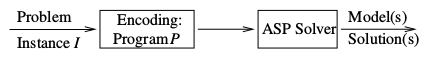
\includegraphics[width=\linewidth]{f1.png}
  \caption{logical steps made in order to find a stable model of a program.}
  \label{fig:ASP1}
\end{figure}
 
Traditional answer set solvers typically have a two level architecture:
\begin{enumerate}
\item Grounding Step: Given a program \(P\) with variables, a (subset) \(P'\) of its grounding is generated which has the same answer sets as \(P\). Grounding is needed because it makes the program smaller and easier to evaluate.
\item Model Search: The answer sets of the grounded (propositional) program \(P'\) are computed. First a candidate model is generated and then stability condition is checked.
\end{enumerate}

There are different techniques for each of the two steps described and their presentation is out of the scope of this paper. For a more detailed explaintion \cite(bho).

\subsection{Hex Programs}
HEX programs \cite{} were introduced as a generalization of  extended logic programs under the answer set semantics. The syntax of HEX programs extend ordinary ASP programs by external atoms, which enable a bidirectional interaction between a program and external sources of computation. External atoms have a list of input parameters (terms or predicate names) and a list of output parameters. Informally, to evaluate an external atom, the reasoner passes the terms and extensions of the predicates in the input tuple to the external source associated with the external atom. The external source computes output tuples that are matched with the output list. Formally, an external atom is of the form \(\&g\:[Y]\:(X)\), where \(Y = Y_1, \dotso , Y_k\) are input parameters the set of terms, variables and predicates and \(X = X_1, \dotso , X_l \) are output terms. 